\documentclass[USenglish]{uit-thesis}

\usepackage[backend=bibtex,style=numeric]{biblatex}
\usepackage{gensymb}
\bibliography{main}

\graphicspath{{images/}}

\begin{document}

%:-------------------------- Frontpage ------------------------

\title{Virtual Reality for the visualization of high-dimensional relationships in bioinformatics}
\subtitle{Subtitle}% Note: this is optional, and may be commented out
\author{\'Alvaro Mart\'inez Fern\'andez}
\thesisfaculty{Faculty of Science and Technology \\ Department of Computer Science}
\thesisprogramme{INF-3990 Master's thesis in Computer Science November 2020}

\maketitle

%:-------------------------- Frontmatter -----------------------
\frontmatter

%: Commented out
\iffalse
\begin{dedication}
To...

Thanks for...
\end{dedication}


\begin{epigraph}
\epigraphitem{Simplicity is prerequisite for reliability.}{Edsger Dijkstra}
\epigraphitem{Beware of bugs in the above code;\\I have only proved it correct, not tried it.}{Donald Knuth}
\end{epigraph}

\begin{abstract}
This is the abstract, blah blah blah.
\end{abstract}

\begin{acknowledgement}
Thank you for blah blah blah
\end{acknowledgement}
\fi
%: End comments

\tableofcontents

%:-------------------------- Mainmatter -----------------------
\mainmatter

\chapter{Introduction}
It is very cheap nowadays to produce data and many people are doing it due to technological advancement. Just as an example, in the field of genomics, the sequencing of the first human genome (2002) took around 13 years and cost over \$3 million to complete. Now we can sequence hundreds of genomes in a few days\cite{big_biological_impacts_bd}. This leads to the accumulation of vast quantities of genomic data, which can be used for new scientific discoveries, diagnose of rare diseases, etc. However we still need a human expert to visually inspect the data to find new signals and discover interesting patterns or to set a diagnosis. No matter how much resources we use into extracting the data if we don't get anything interesting out of it\cite{zhang_paciorkowski_craig_cui_2019}. Therefore there is a great need for new and better tools to support this task.

Some of the main problems that researchers face when analysing genomic data are information overload, data interconnectivity and high dimensionality. One way to deal with all this data is to invent novel analysis. However we still need visual inspection of the data, so the information overload still remains as an important challenge and this is what we attempt to solve. For this reason it is very important to implement efficient visualization technologies that can lead to find new patterns and the extraction of good conclusions of the data. In the field of system biology there are usually network representations where the nodes or bioentities are connected to each other, where these edges represent associations. Networks can increase dramatically in size and complexity and this is due to computational power to create very large networks, scientific knowledge about large networks and the big amounts of data that we have to analyze. We need therefore better visualization systems for the analysis and inspection of these networks.

In Figure \ref{fig:network_biology_evolution} we can see a representation of the evolution for visualization of networks in system biology. Before the computers, networks were represented in 2 dimensions and they were static representations that lacked interactivity, see Figure \ref{fig:network_biology_evolution} A. With the computer era and the advancement in computer graphics, 3D representations were possible, with the addition of interactivity with the network (See Figure  \ref{fig:network_biology_evolution} C). As computer science progressed, there was a big improvement in visualization and also new technologies emerged like virtual reality, which has a huge potential with regards to the interactivity (Figure \ref{fig:network_biology_evolution} I).

\begin{figure}[h!]
    \newlength{\tempheight}
    \setlength{\tempheight}{15ex}
    \centering%
    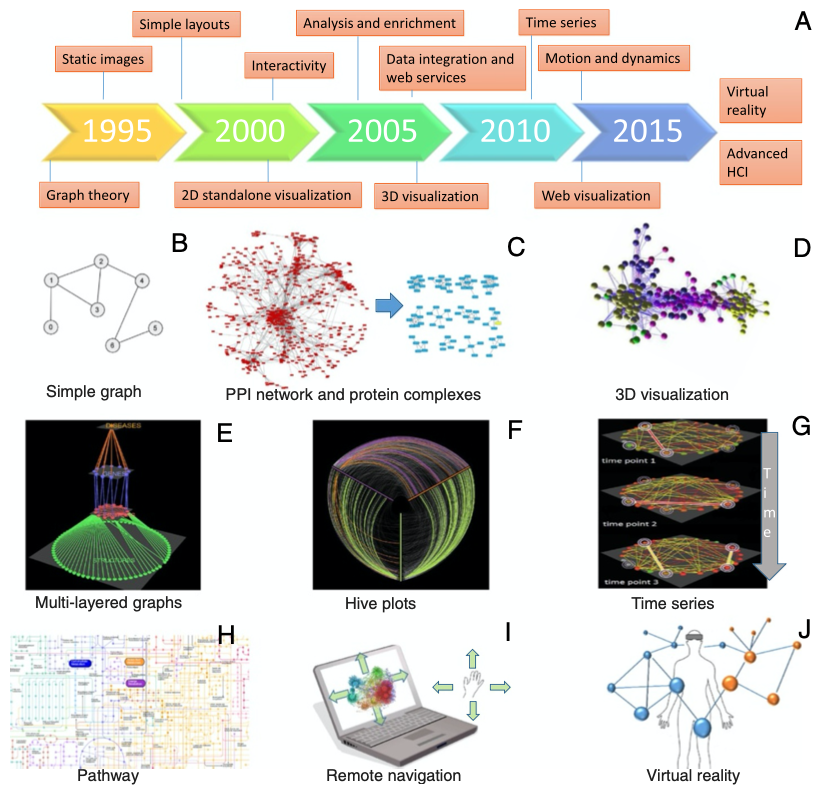
\includegraphics[width=\textwidth]{evolution_visualization}
    \caption{Visualization for network biology. a Undirected unweighted graph showing co-expression relationship between genes. b A 2D representation of a yeast protein-protein interaction network visualized in Cytoscape (left) and potential protein complexes 3D identified by the MCL algorithm from that network (right). c A 3D network of genes showing co-expression relationships. d A multilayered network integrating different types of data visualized by Arena3D. e A hive plot view of a network where nodes are mapped to and positioned on radially distributed linear axes. f Visualization of network changes over time. g Static picture showing part of lung cancer pathway. h Navigation of networks using hand gestures. i Integration and control of 3D networks using VR devices. Figure adapted\cite{pavlopoulos_malliarakis_papanikolaou_theodosiou_enright_iliopoulos_2015}.}
    \label{fig:network_biology_evolution}
\end{figure}%

We believe that virtual reality (VR) can offer new possibilities for visual inspection in large networks. Even though VR is still a field under exploration, it has been demonstrated that it help scientists work more effectively in fields like medicine \cite{Laver11}\cite{xia_ip_samman_wong_gateno_wang_yeung_kot_tideman_2001}\cite{brain_damage_rehab}, biology\cite{10.1093/bioinformatics/bti581}\cite{thorley_lawson_duca_shapiro_2008} and neuroscience\cite{bohil_alicea_biocca_2011}\cite{minderer_harvey_donato_moser_2016}, to  cite some examples. VR can be very powerful because it takes advantage of the way the human being perceives and analysis things. We have a great ability to discover patterns, however we are biologically optimized to see the world and the patterns in 3 dimensions. Some of the advantages that VR has over non-VR approaches are the following:

\begin{enumerate}
  \item Visualization of the network in a 3D space.
  \item Possibility to move around the virtual environment and visualize the network from different perspectives as in real life.
  \item Interaction with the the environment by using controllers and our virtual hands in the virtual world.
\end{enumerate}

We have implemented a virtual reality application for the visualization of 3-dimensional networks of data. We have used  up-to-date virtual reality techniques that we think it improves the visualization of this type of data structures. The techniques that we have used consist in: the exploration of the network by moving around the virtual space, making it easier for the user to see the network from different angles; interaction with the network and nodes to comprehend better the data that is being visualized; and the use of 2-dimensional user interfaces to filter and have more control of the data.

What did we learn... [Write when the evaluation is finished].

\textbf{Thesis statment: } \emph{Virtual reality techniques can improve the visualization and interactivity of data networks.}

\section{Challenges and research problem}
This project focus mainly on solving the problem of visualization of high dimenasional data from the MIxT project by using virtual reality. Furthermore the application allows the user to interact with the network created from the data in the virtual environment. It also allows the user compare the blood and biopsy networks at the same time in order to finde relationship, which wasn't possible in the MIxT web application as this only allows the user to visualize one network at a time.

MIxT\cite{fjukstad_dumeaux_olsen_lund_hallett_bongo_2017} is a web application for bioinformaticians. Among other tools, it offers a network visualization of genes which are represented as nodes in the network and where the edges represent statistically significant correlation in expression between two nodes. This tool was used in a study\cite{dumeaux_fjukstad_interactions_tumor_blood} that identifies genes and pathways in the primary tumor that are tightly linked to genes and pathways in the systemic response of a patient with breast cancer.
When exploring a network in MIxT, it can be hard to understand the data and its relationships because there is too much data. This problem is easy to occur when there are too many node and edges. In figure \ref{fig:mixt_network} we can see an example of the network visualization from MIxT. As we can see in Figure \ref{fig:mixt_network1}, there are many nodes and relationships among them and when we zoom in in the network, it becomes very difficult to understand the data and the relationships as shown in in Figure \ref{fig:mixt_network_zoom}.

 The network is also in 2-dimensions and what we propose in this project is to use a virtual reality 3d visualization in order to cope better with this problem.

\begin{figure}[h!]
    \centering%
    \begin{subfigure}[t]{0.5\textwidth}
        \centering%
        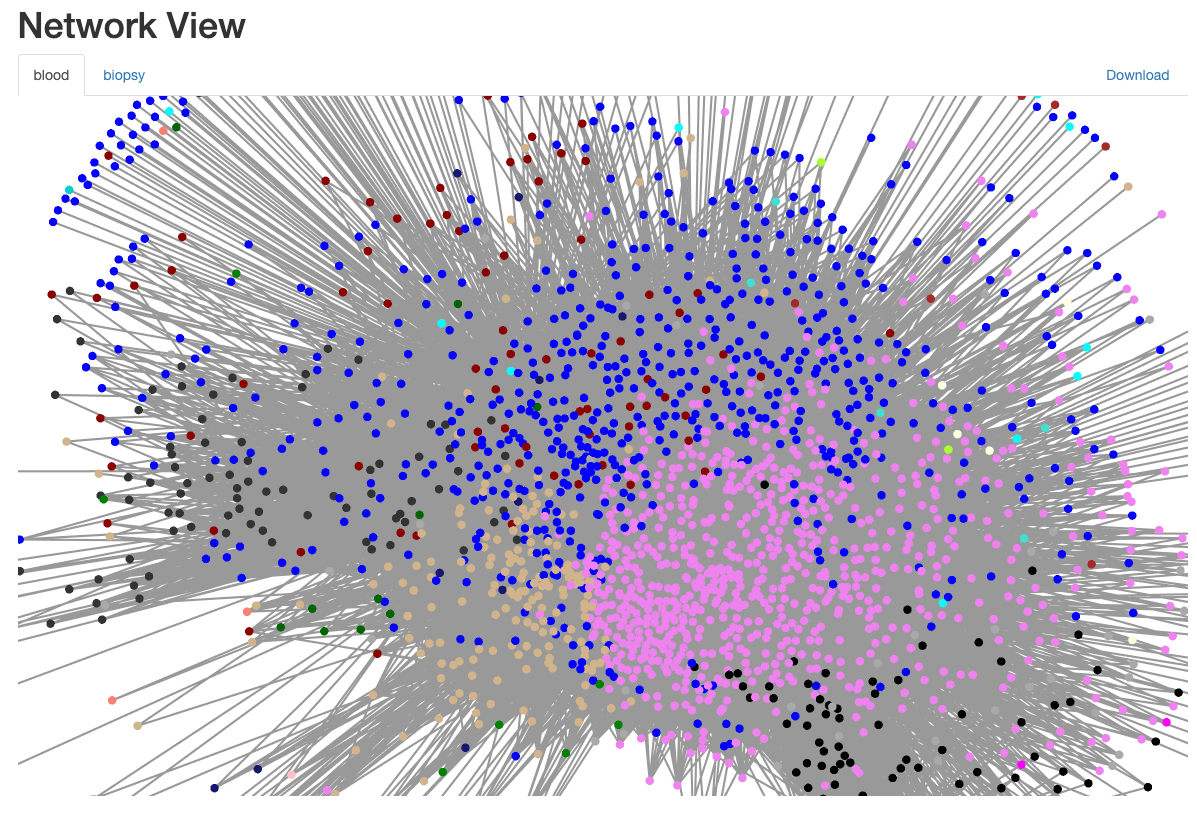
\includegraphics[width=\linewidth]{mixt_network1}
        \caption{Network with several modules.}
        \label{fig:mixt_network1}
    \end{subfigure}%
    \begin{subfigure}[t]{0.5\textwidth}
        \centering%
        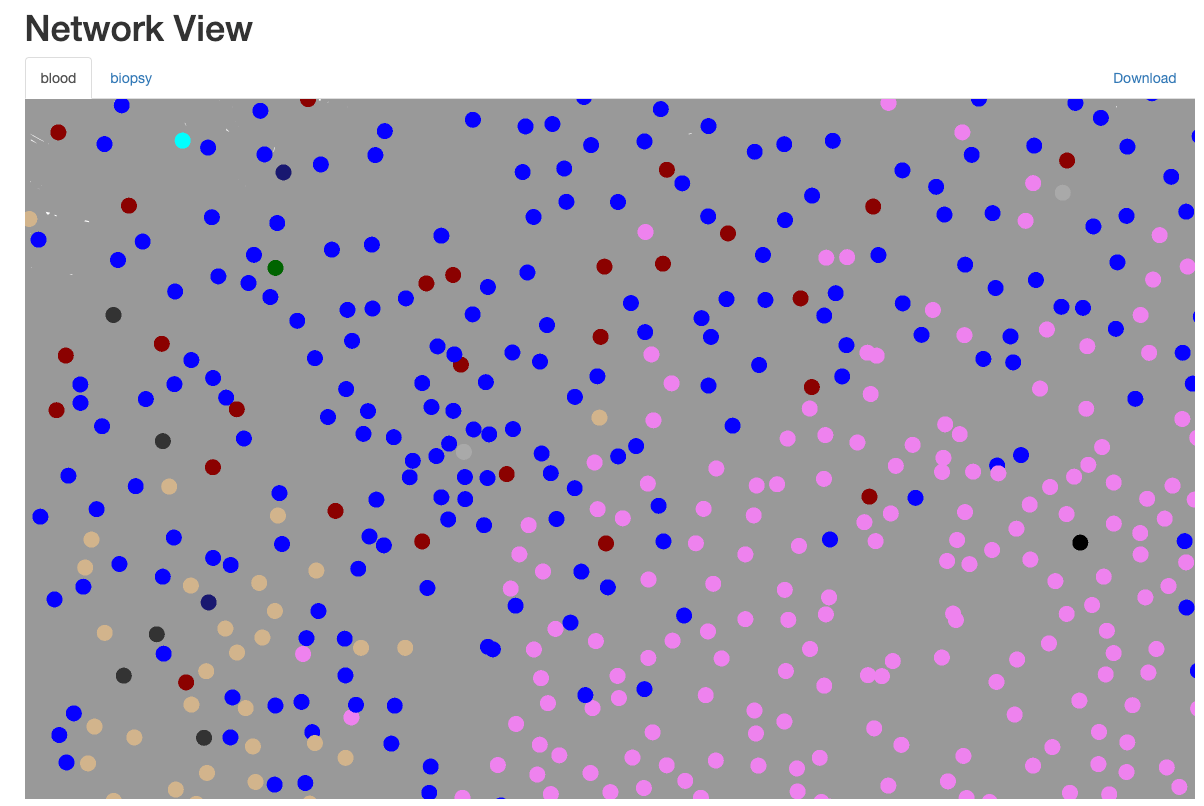
\includegraphics[width=\linewidth]{mixt_network2}
        \caption{Zoom in the network.}
        \label{fig:mixt_network_zoom}
    \end{subfigure}

    \caption{Network view of the MIxT application where nodes repsent genes and the modules are repsented by colors. Relationships are represented by grey lines that connect a gene with another one.}
    \label{fig:mixt_network}
\end{figure}

\section{Proposed solution}

\section{Significance and contribution}
This project contributes in the exploration of the possibilities that Virtual Reality offers for visualization of big data in bioinformatics.

\section{Outline}


\chapter{BigNet VR}
%
% The points that I want to cover are the following:
%
% \begin{itemize}
%   \item Building the network from the bioinformatics data and clustering.
%   \item Manipulation of the network: translation and scaling.
%   \item Locomotion and ergonomics used in the VR environment.
%   \item Changing from the blood network to the biopsy network and viceversa.
%   \item Filtering genes in the network using gene sets that represent signatures of cellular pathways which are often dis-regulated in cancer.
% \end{itemize}

%In order to explore the network, several features have been implemented with the purpose of enhance the experience of the visualization process. For example the user has the possibility to move around the network by teleporting to a different place. It is also possible to translate the network and scale it, allowing the user have a better view of the data. The user can also point at a node using the controller to show the name corresponding to that gene or node. Another feature is about entering into a menu where the user can filter the network according to gene sets that represent signatures of cellular pathways which are often dis-regulated in cancer. And finally it is possible also to switch the network from a blood dataset to a biopsy dataset and viceversa.

%The genes nodes in the network and are represented as squared dots and the relationships are represented with lines between them. In Figure \ref{fig:bignet_vr} we can see an example of the application running.

BigNet VR is a virtual reality application for the interactive visualization of large-scale networks in a 3D space. The network is represented using nodes and connections between them. In order to explore and visualize the data in BigNet VR, the user can walk around the 3D environment, scale the network, translate it to other places, filter the nodes using a user interface and also obtain detail information about the data.

BigNet VR works with a dataset that contains the information of the nodes and relationships that make up the network. This dataset needs to be obtained from an external source. Once we have our dataset we can load it to the application and then run it using a HMD (Head Mounted Display) for VR. Finally we can explore the network and interact with it to visualize the dataset in a VR experience.

The implementation of BigNet VR is carried out in Unity, a cross-platform game engine. This software is used for a wide range of applications, especially for the development of videogames in 3D and 2D, VR applications and engineering solutions. The programming language used to develop the application inside Unity is C\#. We also used VRTK, a VR toolkit to build VR solutions in Unity. As for the VR hardware, we used an Oculus Quest headset. This type of headset is an oll-in-one HMD, which means that it doesn't need to be connected to a PC to run an application, it can be run inside the hardware of the headset itself. However during the development process, the headset needs to be connected to the PC and the application can be run and tested directly from Unity.

For this chapter we will use dataset examples from MIxT to illustrate the concepts that we will talk about. MIxT is a web application that is used for the visualization of bioinformatic data\cite{fjukstad_dumeaux_olsen_lund_hallett_bongo_2017}\cite{dumeaux_fjukstad_interactions_tumor_blood} and the datasets used here contain genetic information about a woman with breast cancer. There are in total 2 datasets; the first one is from a blood sample and the second one is from the tumor sample. In Figure \ref{fig:bignet_vr} we can see an example of the application running using the blood dataset from MIxT.

\begin{figure}[h!]
    \setlength{\tempheight}{15ex}
    \centering
    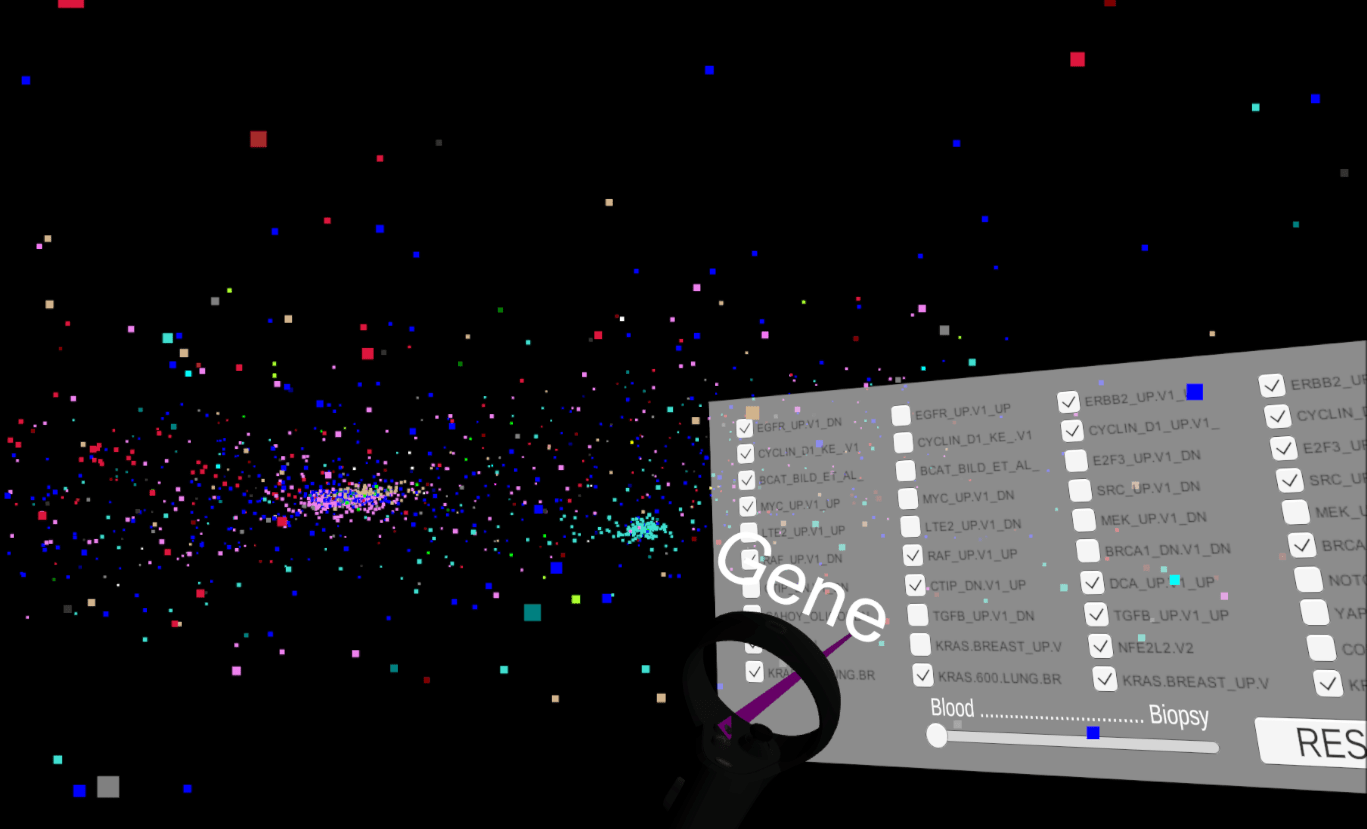
\includegraphics[width=\textwidth]{bignet_vr}
    \caption{BigNet VR. Example of the application running on a Oculus Quest.}
    \label{fig:bignet_vr}
\end{figure}

\section{Visualization and interaction with the network}
Virtual reality headsets offer a rich inmmersive experience. It's not only about inmersing the user into a 3D environment, but also giving the user the possibility to interact with the environment itself. This makes it possible to build complex VR applications where the user can do almost anything in a virtual world. Some examples of what is possible to do in virtual reality is for example moving around, grabbing objects, interact with the environment using your hands or virtual tools, 2D interfaces and menus, etc. In this section we will explain the techniques that we have implemented to visualize and interact with the network and make the most of VR. These techniques correspond to how the user can move around in the network and how the user can visualize the data.

Oculus Quest is an all-in-one VR headset and so it doesn't need a PC nor wires to run the applications. Apart from the headset, it comes with 2 controllers; one for each hand. These controllers have inputs as buttons, thumbsticks and triggers that can be used to activate actions in the VR application. We have used some of these inputs available in the controllers in BigNet VR and mapped them to different actions that allow the user interact with the network and the environment. In Figure \ref{fig:oculus_quest_inputs} we can see which actions correspond to each input from the controllers. We will explain now the different methods that we use in BigNet VR to visualize the data and how we can enable them using the controllers.

\begin{figure}[h!]
    \centering%
    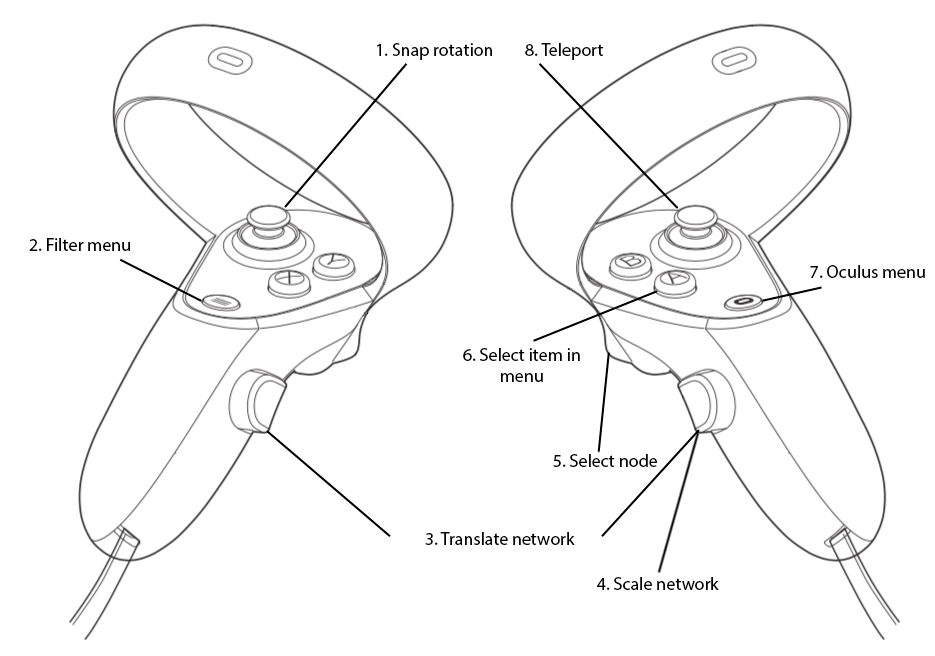
\includegraphics[width=\textwidth]{oculus_quest_inputs}
    \caption{Mapping of the Oculus Quest controllers for the different actions implemented in BigNet VR: 1. Snap rotation. 2. Filter menu. 3. Scale environment. 4. Translate environment. 5. Select item in menu. 6. Oculus menu. 7. Teleport. Adapted figure from Oculus developer's page\cite{oculus_inputs}.}
    \label{fig:oculus_quest_inputs}
\end{figure}%

\subsection{Locomotion}
Locomotion is one of the most important ways of interaction in virtual reality experiences. It can be defined as a self-proppelled movement in the virtual world. Even though moving around is not the main goal in most of VR applications, it is an important aspect for the user's perspective in order to move the user's viewpoint in the virtual world and navigate around it.

Locomotion can have an strong influence in the user's experience. A poorly designed locomotion technique can reduce the user's immersion and even introduce motion sickness, which is related to the movement that the technique produces. HMDs like Oculus Quest allow the users to control the position and the orientation of the viewpoint by moving their heads and walking. However large virtual environments such as BigNet VR need a big physical tracked area which cannot be covered by just walking around. It is for this reason that we need to use a locomotion technique that makes it possible to move around without the having to walk\cite{locomotion_technique}.

The locomotion technique that we use in BigNet VR is called teleportation. It consists in choosing a spot on the floor were we want to teleport to. To do this the user has to move forward the thumbstick from the right controller (see "7. Teleport" from Figure \ref{fig:oculus_quest_inputs}). In addition it is possible to choose which direction the user will face once the teleportation is completed. To do this we just need to rotate the same thumbstick to the desired direction. Once the user releases the thumbstick, a black flash will be followed by the new position in the space. This black flash is very important when implementing some techniques because it prevents from producing motion sickness and disorientation.

\begin{figure}[h!]
    \centering%
    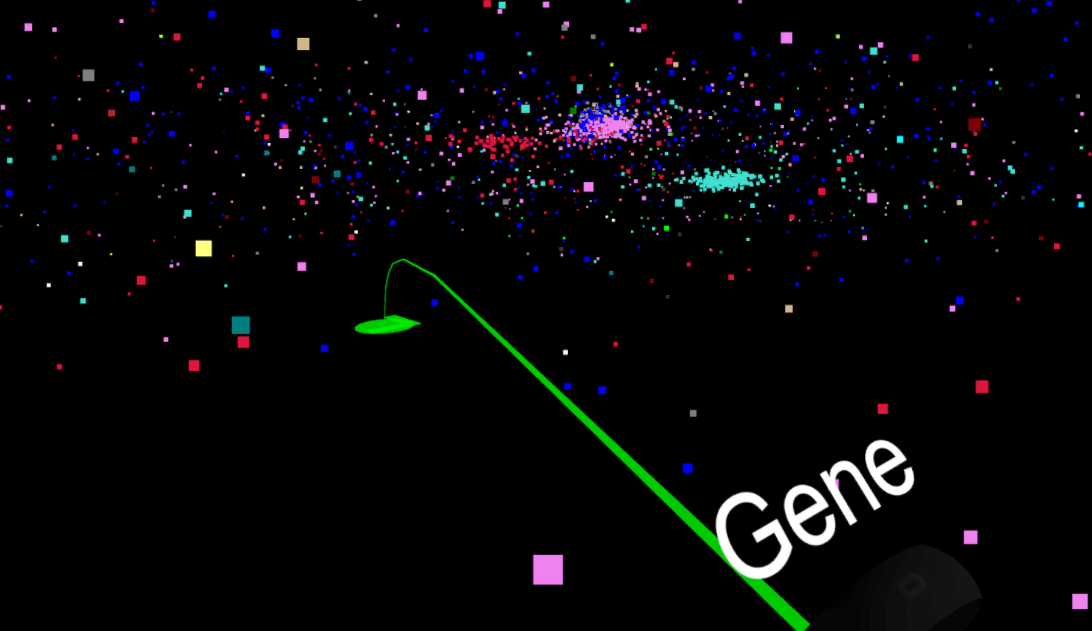
\includegraphics[width=\textwidth]{teleportation2}
    \caption{Teleportation technique. The user can use the jystick from the right controller to teleport to a different spot. To choose the spot a parabolic arc will appear.}
    \label{fig:teleportation}
\end{figure}%

In Figure \ref{fig:teleportation} we can see an example of how the teleportation technique is used in BigNet VR. A  parabolic arc is created in the 3D space with a circle representing the teleporting place. It can be seen as if we are throwing an object to the spot where we want to teleport to. The green circle includes also an arrow, indicating the direction that we will face once we are teleported.

In addition to the teleportation, we have also added the possibility to rotate to the left or to the right so that the user doesn't need to rotate the head too much. This action is triggered using the thumbstick on the left hand (See 1. Snap rotation in Figure \ref{fig:oculus_quest_inputs}). By moving the thumstick to the left side, the camera will rotate 45$^{\circ}$ to the left side, and 45$^{\circ}$ to the right side if the user moves it to the right side. A black transition is also used in this case before the rotation happens to avoid motion sickness.

\subsection{Translation of the network}
By teleporting to different places in the environment we allow the user see the network from different perspectives. However it is also interesting being able to move the network and specially move in a precise way so that the user has more control over what it is being visualized. The user might for instance be able to see the network or a specific node or cluster from above or also from below. To do this we have implemented a functionality to translate the network in the 3D space.

\begin{figure}[h!]
    \centering%
    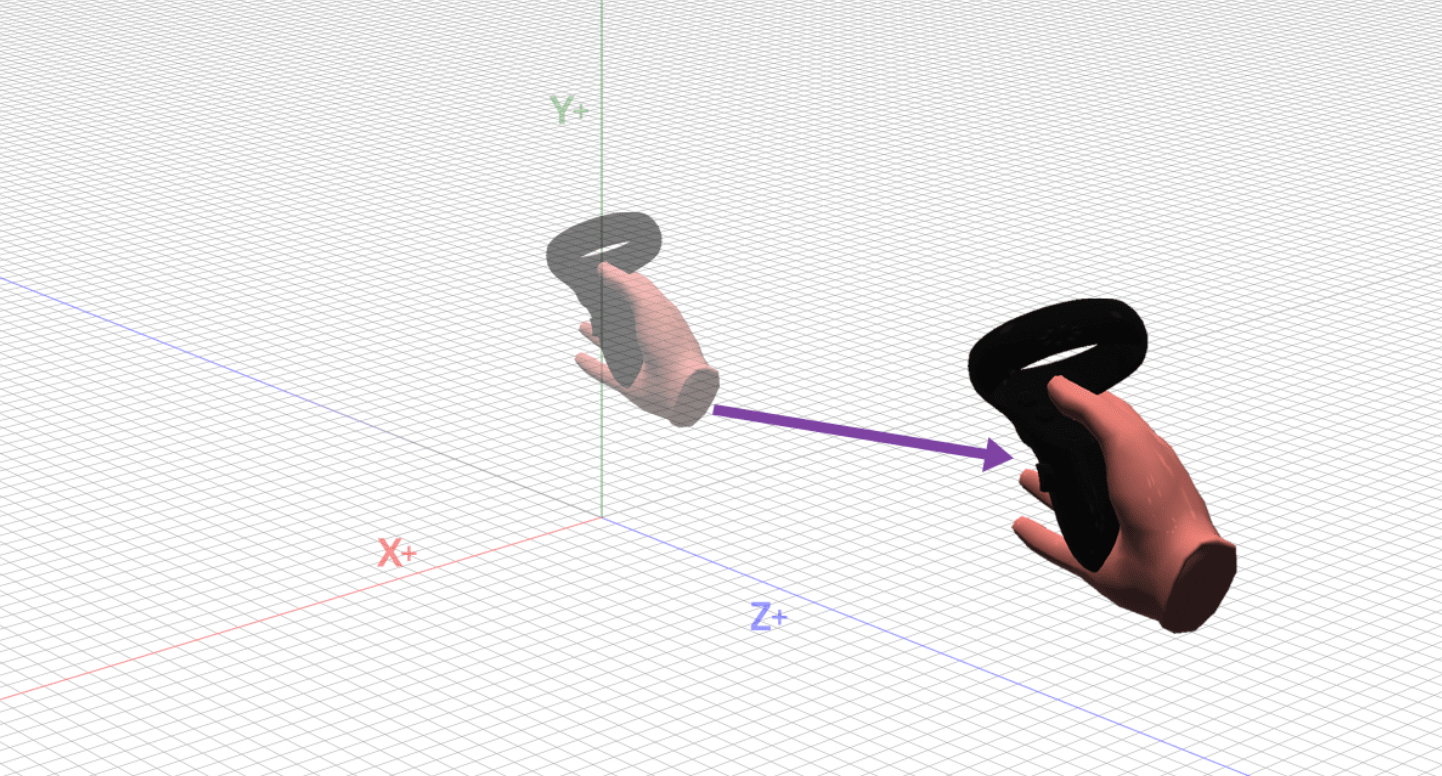
\includegraphics[width=\textwidth]{translation}
    \caption{Translation of the network functionality. The user holds the translation button on the Oculus controller and moves the hand to the direction where he or she wants the network to translate.}
    \label{fig:translation}
\end{figure}%

To translate the network in BigNet VR, the user needs to press on the hand trigger from the right controller (see "4. Translate environment" in Figure \ref{fig:oculus_quest_inputs}). Then the user needs to keep holding this trigger down and move the hand to the direction to which we want the network to move to. This intuitive approach feels like we are just pulling from a rope tied to the network and we just move it to the direction we want.


\subsection{Zooming in the network}
When exploring a big network with hundreds of nodes and several clusters, sometimes the information can be too crowded. In our example dataset that we use in BigNet VR, there are some clusters of nodes that have too many nodes close to each other and it gets very hard to visualize them properly. A way to cope with this problem is for instance by "zooming" in the part of the network that we want to explore better. We implement then a scaling functionality that makes the network bigger or smaller.

The way we implemented the zooming functionality in BigNet VR is by using the hand triggers with the name "3. Scale environment" (see the reference in Figure \ref{fig:oculus_quest_inputs}). In the first place the user needs to press and hold these triggers from both controllers and then we need to expand or contract the arms, as if we were streching out or contracting the network itself. This is also an intuitive acction to do since the user might think that we are actually stretching the network with the hands.

\begin{figure}[h!]
    \centering%
    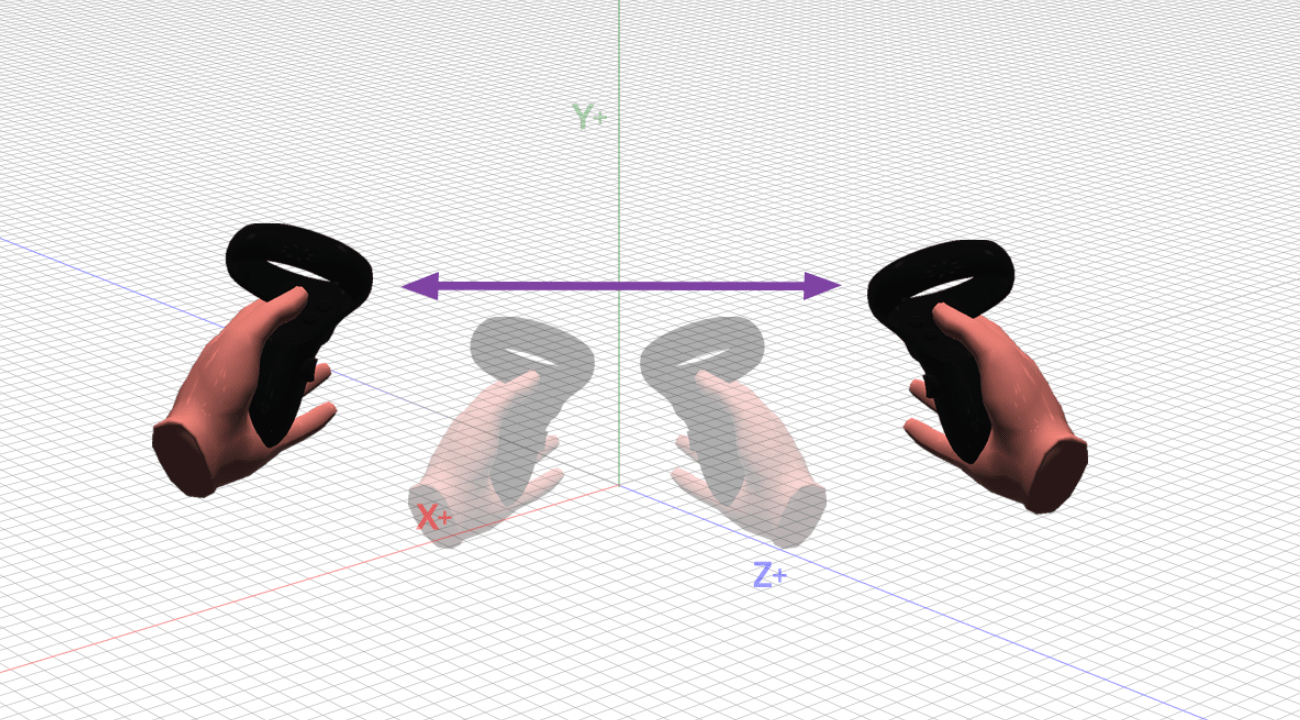
\includegraphics[width=\textwidth]{scaling}
    \caption{Zooming in the network functionality. The user can hold the scaling buttons on the Oculus controller to make the network bigger or smaller. In this example if we strech our hands outside, the network will expand.}
    \label{fig:scaling}
\end{figure}%


In Figure \ref{fig:scaling} there is a visual example of how the zooming works using the Oculus controllers. In this example the user is stretching the hands out in order to make the network bigger. The user starts in a intial position, then holds the zooming triggers from both controllers and then moves the hands out. If we wanted to make the network smaller we would do the opposite action, by contracting the hands to the inside.

\subsection{Interaction with the nodes}
BigNet VR provides also detailed information about the data that is being displayed. The user can interact with the nodes of the network to obtain information about ecah of them. In our example, the nodes represent genes and the user might be interested in knowing which gene name corresponds to a specific node. The action that we need to do to obtain the name of the gene is to point at the node that we are interested in and press the "5. pointer" index trigger on the right controller (see Figure \ref{fig:oculus_quest_inputs}). When we press this trigger, a laser pointer will appear from the virtual controller inside of the application. By pointing to a specific node with the pointer, we will get the name of that gene node that will be displayed in a rendered text.

[User figure showing how the pointer works and explain it. This part of the implementation needs to be improved.]

\subsection{Node relationships}
Finally, our dataset has information about the relationships between the nodes. BigNet VR is implemented to show also this information. Because there can be many relationships in the dataset we don't show them all at the same time. We can only see those of the nodes that are close to the user. The way that these relationships are represented is with lines between the nodes. These lines disappear once the user moves away from the nodes.

[User figure showing how the relationships are shown in the application and explain the example. This part of the implementation needs to be improved.]


\section{Building the network}
BigNet VR uses a datasets that has been created from a external source to build the network. The datasets have to be in CSV format and we need 2 datasets in total to build the network. The first one contains the information about the categories and the nodes that belong to each category and the second dataset has information about the relationships between each of the nodes.

The following diagram in Figure \ref{fig:create_network} explains in a broad way what steps we follow to build the network in Unity. We start with the 2 datasets described before, containing the data for the network. We process the dataset with information about the categories and build a particle system object in Unity, where each particle corresponds to a node. We also add to each particle a color, which is related to the category that the particle belongs to. Finally we apply a cluster algorithm using the data from the dataset with information about the relationships.

\begin{figure}[h!]
    \centering%
    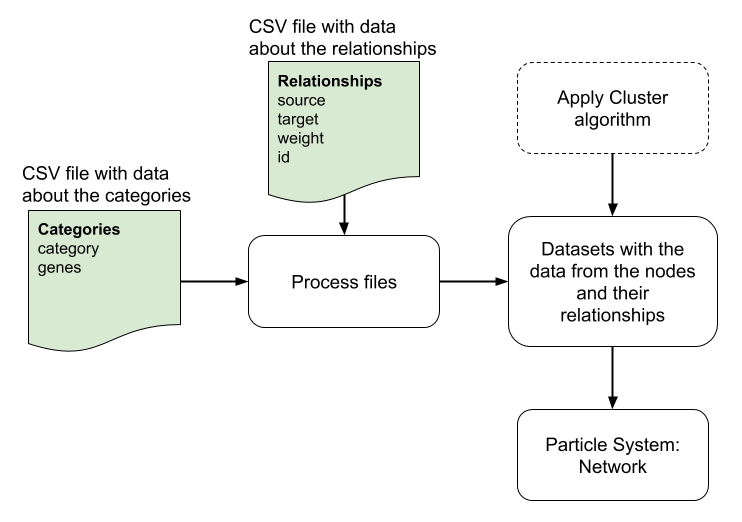
\includegraphics[width=\textwidth]{create_network}
    \caption{Diagram explaining how the network is built in Unity.}
    \label{fig:create_network}
\end{figure}%

Following our bioinformatic network example, in Table \ref{tab:categories-data} and Table \ref{tab:network-data} we show an extract of how the datasets look like. Table \ref{tab:categories-data} has the data about the nodes or genes in this case and the categories to which each node belongs to. These categories are named by colors and these color names will be used by BigNet VR to color each particle of the particle system. Then in Table \ref{tab:network-data} we have the information about the relationships. This dataset can be very extend because each row of the CSV file corresponds to a relationship between 2 nodes or genes in this case and one gene can be connected to many other nodes.

\begin{table}[h!]
\centering
\begin{tabular}{ll}
\hline
category & genes          \\
brown   & ARHGAP30 FERMT3 ARHGAP25 CD53 PLEK IRF8 DOCK2\\
cyan  & SAFB MOB3A RAB35 ABR ASCC2 CDC37 ANKFY1 GLTSCR1\\
darkgrey  & RAB40C ZNF213 ZNF263 PIGQ RHBDF1 RAB11FIP3\\
darkorange  & TCEB1 MRPL13 ENY2 MTERF3 UBE2W WDYHV1\\
\hline
\end{tabular}
\caption{Fragment of the dataset with the categories and the genes belonging to each category from the biopsy sample.}
\label{tab:categories-data}
\end{table}

\begin{table}[h!]
\centering
\begin{tabular}{llll}
\hline
source & target & weight            & id          \\
AAMP   & ARGLU1 & 0.102486209330144 & AAMP-ARGLU1 \\
ACADM  & FOXN2  & 0.107506881676173 & ACADM-FOXN2 \\
ACADM  & MBNL1  & 0.12269622045714  & ACADM-MBNL1 \\
ACADM  & PPM1B  & 0.103496640767895 & ACADM-PPM1B \\
\hline
\end{tabular}
\caption{Fragment of the dataset used to build the network relationships of the blood sample.}
\label{tab:network-data}
\end{table}

\section{Filtering information in the network}
Another feature that BigNet VR uses to improve the visualization of networks is a filtering menu. When we have huge amounts of data in large networks, it is sometimes necessary to show less or more data. By filtering the nodes we can visualize only the part that we are interesting in.


\begin{figure}[h!]
    \centering%
    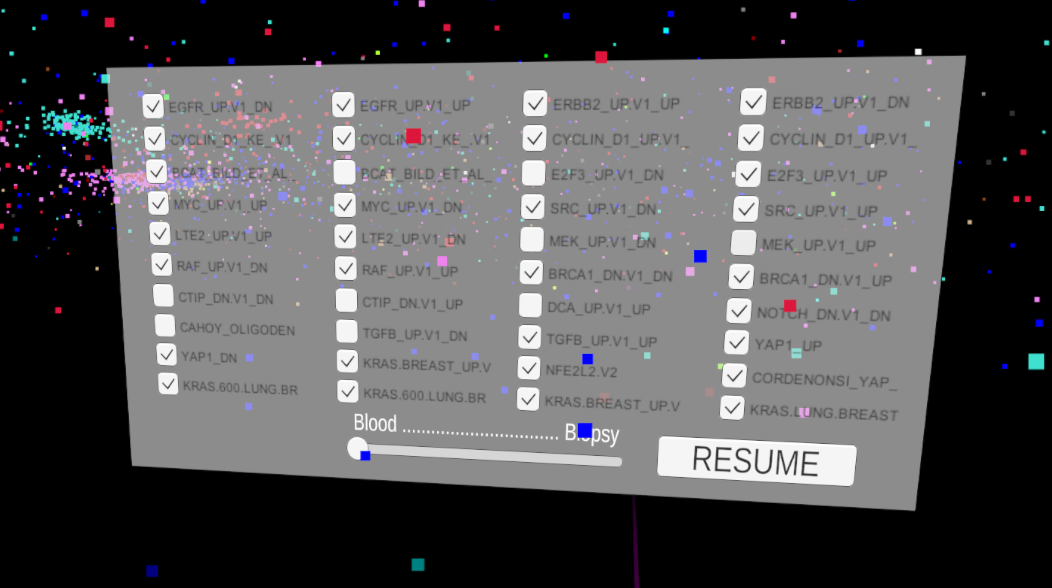
\includegraphics[width=\textwidth]{filtering}
    \caption{Filtering menu in BigNet VR.}
    \label{fig:filtering}
\end{figure}%


We have built a 2 dimensional menu in Unity, see Figure \ref{fig:filtering}, to filter the data in our example network. We use checkboxes for the filtering. From a starting point, all the boxes are checked, and if the user wants to hide a part from the visualization it is done by unchecking the box. To show the filtering menu we need to press on the menu botton from the left controller, see the "2. Filter menu" in Figure \ref{fig:oculus_quest_inputs}. The to check or uncheck the boxes we need to use the A botton from the right controller, named "6. Select item", see Figure \ref{fig:oculus_quest_inputs}.

\section{Switching dataset}
Finally BigNet VR has also the possibility to switch between datasets. This can be done in the filtering menu by pressing the menu button from the left controller and there we can see a slider UI element as in Figure \ref{fig:filtering} which we can move to the right or to the left in order to change the dataset that is being visualized. When we switch the dataset, the filters are also reset to their default state, so all of them will be checked in our example. In our bioinformatic usecase we can switch from the blood dataset to the biopsy one.


\chapter{Related work}
I will focuse in this chapter on VR applications found in the literature for the visualization of bioinformatic data.

\section{Virtual Reality Chemical Space}
Virtual Reality Chemical Space is a VR application for the interactive exploartion of chemical space populated by Drugbank compounds\cite{drugbank}. It is also developed in Unity using C\# and the VRTK library. They use a particle system to render the particles of the chemical space. To render the particles, they use shaders instead of geometrical spheres as well, optimizing the number of vertices per datapoint in the scene. In order to reduce the motion sickness they have introduced a floor in the form of a grid acting as a static frame of reference. Also instead of letting the user move through the VR environment, they use a controller to move the point cloud. In Figure \ref{fig:drugbank} we can see an screenshot from the VR application. As we can notice in the screenshot, there is a subtle rendering of an outer space scene as an independent visual background. This is another technique to reduce the motion sickness that helps the user keep the notion of space. This is an interesting technique that we could have tried in BigNet VR.

They conclude in the article that the application that they have developed doesn't visualize an environment with an analogue in the real world, but instead a mathematical construct. Also some of the drawbacks that VR has compared to traditional solutions is that the VR headsets are not so comfortable as well as often-occurring eye strain and virtual reality sickness. They also conlcude that the application of VR in chemistry has more potential in the fields of education and training as for the current state of technology. The tools for chemistry need to be further evaluated wether they should be extended to VR.

\begin{figure}[h!]
    \centering%
    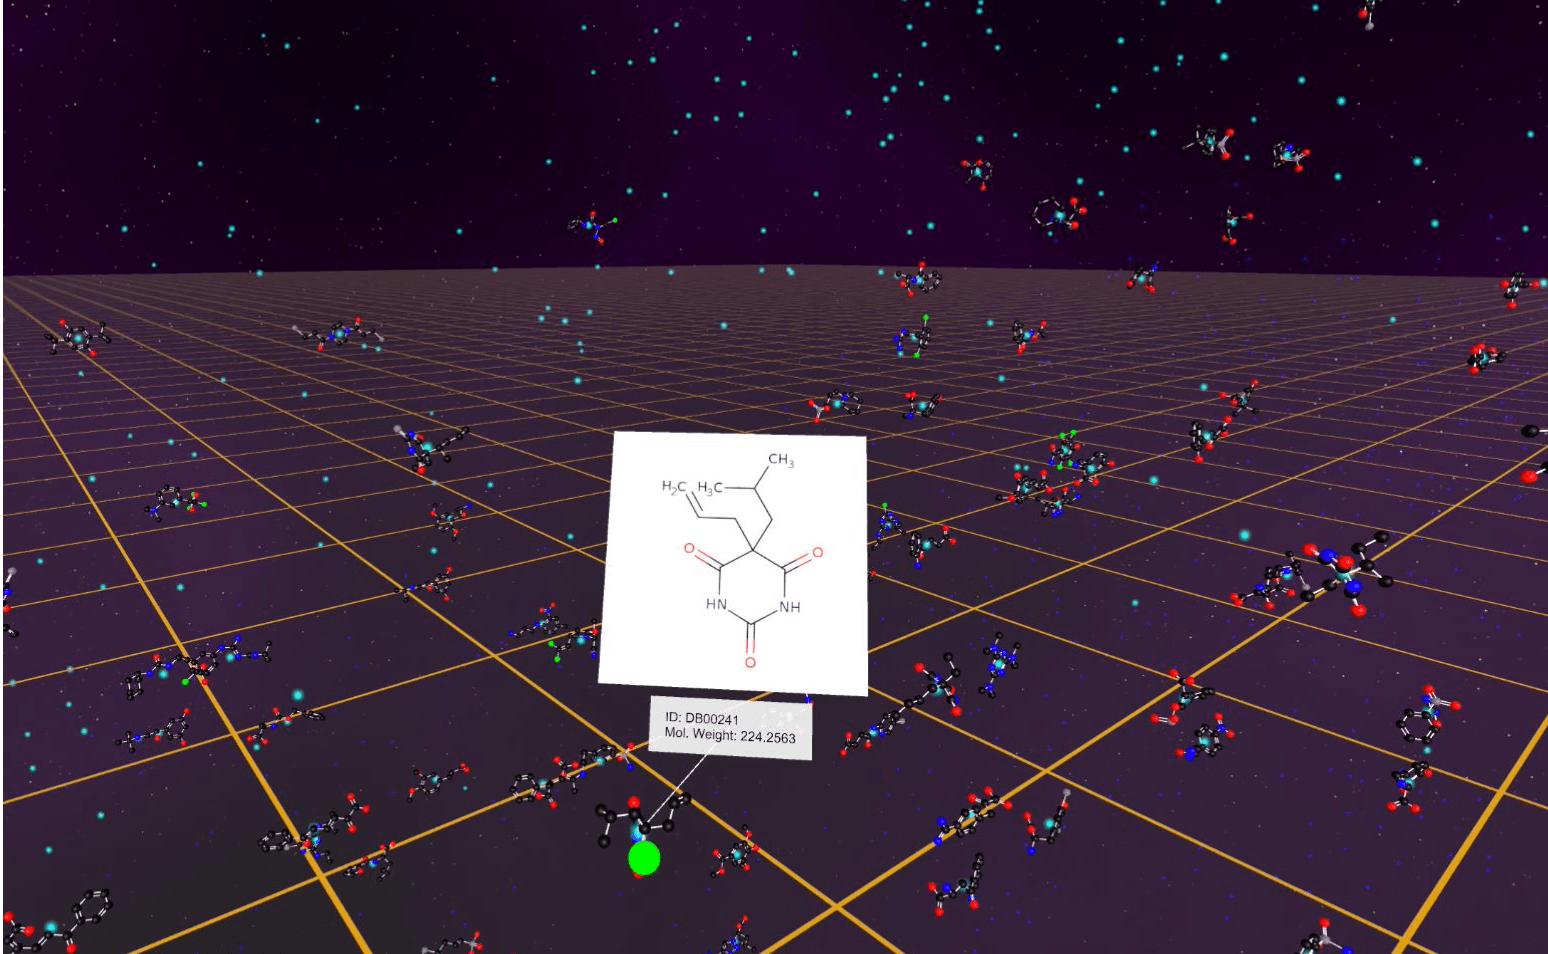
\includegraphics[width=\textwidth]{drugbank}
    \caption{Optimized virtual reality chemical space. Figure taken from \cite{drugbank}.}
    \label{fig:drugbank}
\end{figure}%

\section{BioVR}
BioVR is an interactive VR platform for integrated visual analysis of DNA/RNA protein structures\cite{biovr}. It is built in Unity and using C\#. The headset that they targeted the application to is Oculus Rift. One big difference between BioVR and our application is that in BioVR they use the hands for the interactions rather than the controllers. This can be very attractive and it could have worked very well for BigNet VR, since most of the interactions can be done with hand gestures. Also since early 2020, hand tracking has been integrated in Oculus Quest, making it easier for dveleopment\footnote{https://developer.oculus.com/documentation/unity/unity-handtracking}.
An screenshot of BioVR can be seen in Figure \ref{fig:biovr}. The user in BioVR can visualize the virtual hands in the virtual world and they are used for the interaction with the nucleotide sequence and UI menus. In BigNet VR instead of the hands we show the controllers, which help the user orientate in the space. The research concludes that using VR helps in create new workflows for researchers to view DNA/RNA sequence and protein structures. They also  of VR is that it is easy to integrate 2D user interfaces in the virtual world, as we can see in Figure \ref{fig:biovr} B.

\begin{figure}[h!]
    \centering%
    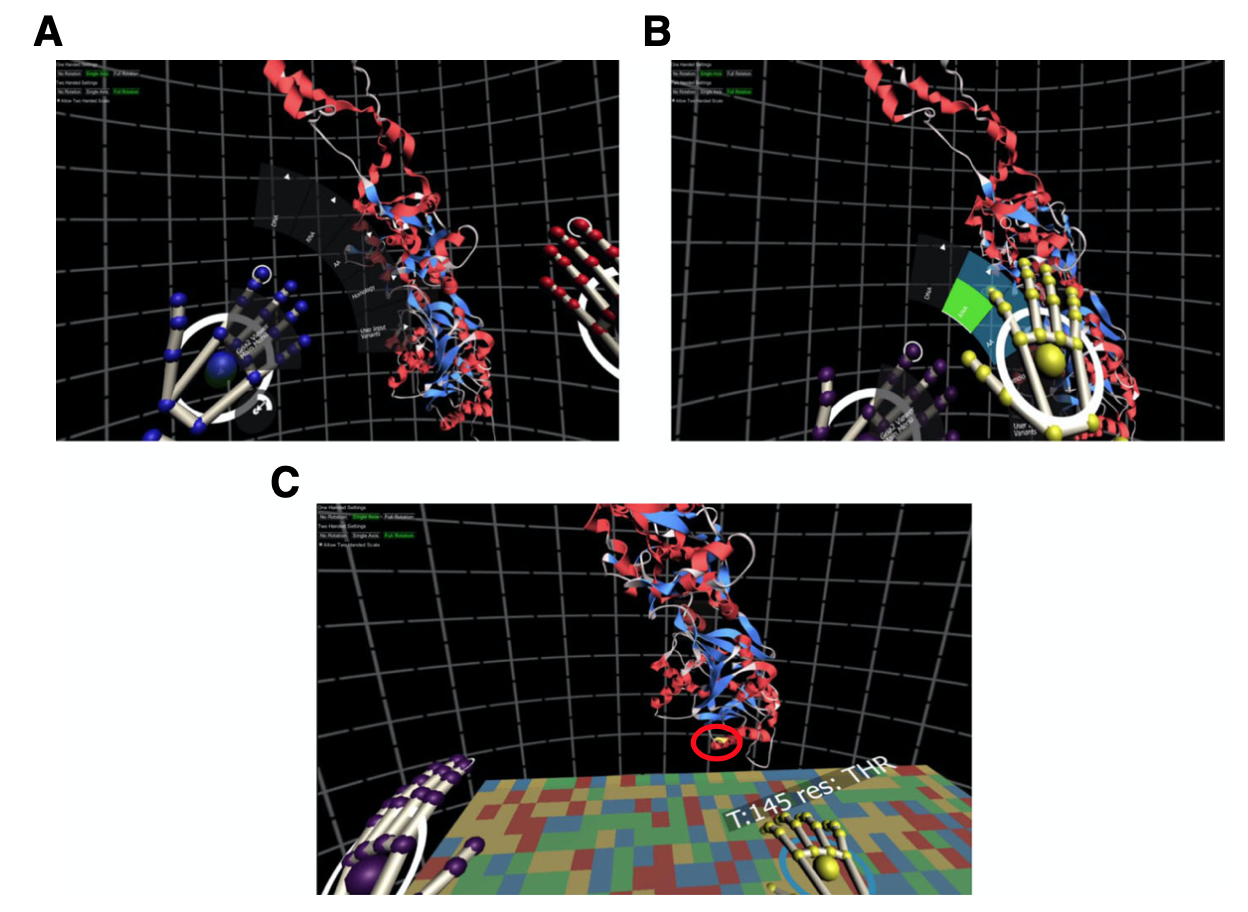
\includegraphics[width=\textwidth]{biovr}
    \caption{Screenshot from BioVR. Figure taken from \cite{biovr}.}
    \label{fig:biovr}
\end{figure}%

\section{CellexalVR}
CellexalVR is a virtual reality envirnoment for the visualization and analysis of single-cell RNAseq experiments that help researchers undertand their data\cite{cellexalvr}. The system is divided in two parts: the first one consists on the VR interface and the second is an R package called cellexalvrR that does back-end calculations and also provides functions that allows the user export the scRNAseq data from an R session for CellexalVR to read. CellexalVR was developed in Unity for HTC Vive (Pro). They used Unity and C\# and R for the implementation. They used libraries like VRTK, OpenVR and SteamVR as well in the implemenation.

Something that is interesting in CellexalVR is that it allows a multi-user mode via the Photon Unity Networking. This works sending information about the events to each user using Remote Procedure Calls. In Figure \ref{cellexavr} we can see an screenshot from CellexalVR where two users participate in the same session. Other users can also be in the same session but just be watchers and be in like a "ghost mode". This is something interesting that could be used in BigNet VR as well. Espcially the "ghost mode" could be useful so that other people can visualize the network at the same time from other perspectives.

\begin{figure}[h!]
    \centering%
    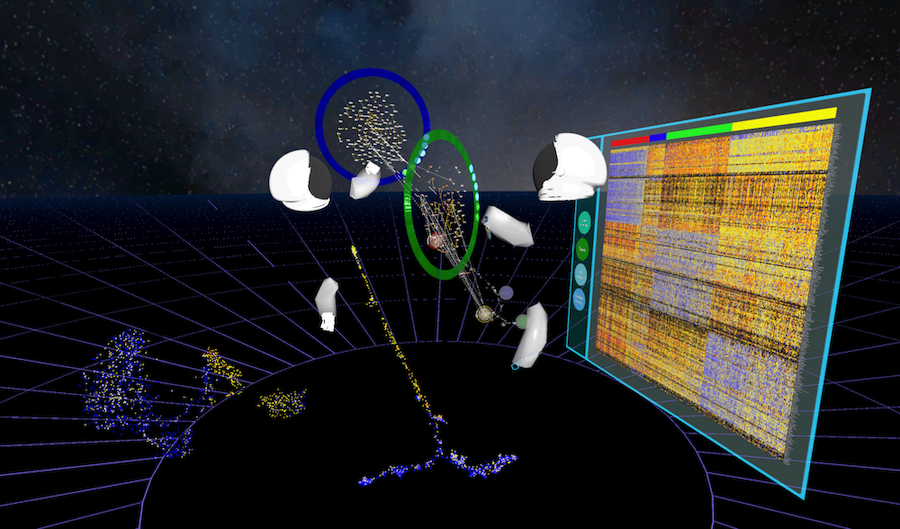
\includegraphics[width=\textwidth]{cellexavr}
    \caption{Screenshot from CellexalVR. Two users using CellexalVR at the same time. The head models were taken from NASA. Figure taken from \cite{cellexalvr}.}
    \label{fig:cellexavr}
\end{figure}%

\section{BigTop}
BigTop is a visualization framework in VR for the rendering of Manhattan plots in three dimensions\cite{bigtop}. Manhattan plots are usually 2-dimensionals, where genomic coordinates are displayed in the x-axis and the negative log-10 of the association P-value for each single nucleotide polymorphism (SNP) displayed on the Y-axis. Each dot on the Manhattan plot signifies a SNP then. In BigTop, the z-axis is used to display minor allele frequency of each SNP. This allows the identification of allelic variants of genes. As for the interaction, BigTop allows the user to select a node in order to obtain more information like the SNP name. BigTop is built in JavaScript with the React and A-Frame frameworks. It can also be rendered in any commercially available VR headsets and also in 2D web browsers.

To move around the scene in BigTop the user can take steps (in the VR version) or using the arrow keys from the keyboard. The user can select the nodes by pointing with a laser at the nodes in the scene in the VR version. In the browser version it is possible to select them using the pointer from the mouse. Also in order to look around, the user needs to move the head around using the VR headset, or by isong click and drag with the mouse (in the browser). In BigNet VR we have focused only into building a visualization system for a VR headset. We have used better locomotion techniques that improves the comfortability. However the locomotion technique that they use to move around could be a good idea for BigNet VR as well.

\begin{figure}[h!]
    \centering%
    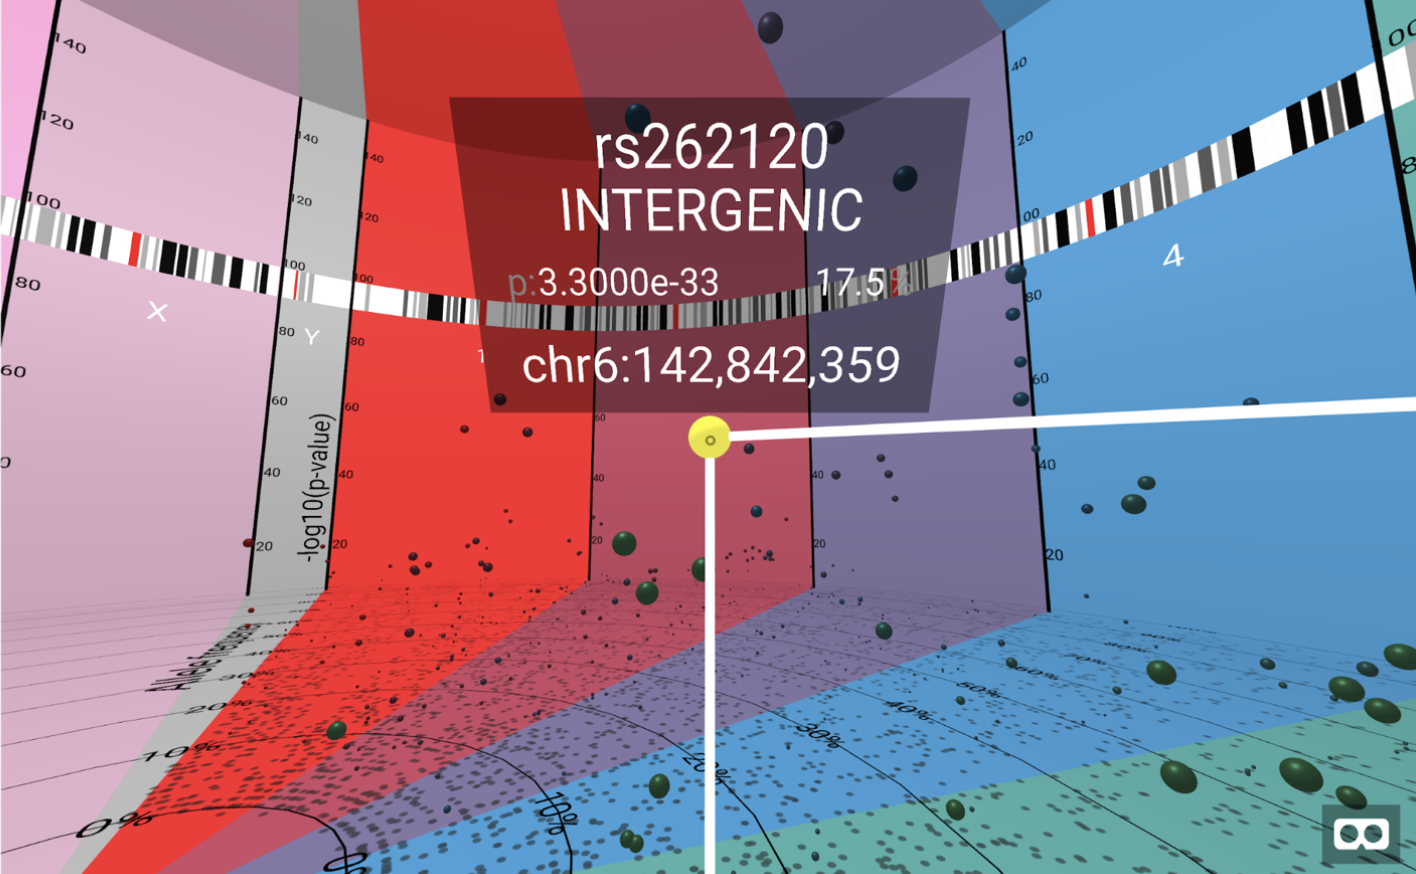
\includegraphics[width=\textwidth]{bigtop}
    \caption{Screenshot from BigTop. Figure taken from \cite{bigtop}.}
    \label{fig:bigtop}
\end{figure}%


\chapter{Evaluation and discussion}
% Benchmarking in Unity
% https://blogs.unity3d.com/2018/09/25/performance-benchmarking-in-unity-how-to-get-started/
% Maybe try VRWorks https://developer.nvidia.com/vrworks

% Questions to answer in the evaluation chapter:
% \begin{enumerate}
%   \item{How big can the graph be so that it is comfortable visualizing the network?}\\
%   What is comfortable? Number of FPS?
%   How can we scale the graph? By adding nodes and spread them around, by adding more interconnexions?
%   Should the experiment split in several parts? Scaling, filtering, moving around, etc.
%   What is the performance by using Oculus Link and the performance using just the Quest hardware?
%   -We can use the Unity GPU Profiler for Oculus Quest and Go in order to see the performance.\\
%   \href{https://developer.oculus.com/blog/getting-started-w-the-unity-gpu-profiler-for-oculus-quest-and-go/}{See: Getting Started w/ The Unity GPU Profiler for Oculus Quest and Go}
%   \item{How is this way of visualizing the graph better by using VR?}\\
%   We are researchging the technology and the test with actual users is for future work.
%   \item{In what way can the application and the visualization of the graph be improved?}\\
%   Argue in the discussion part.
% \end{enumerate}

% Links
% Profiler panel

BigNet VR has been implemented to explore biological networks like the one from MIxT. In this chapter we will evaluate the scalability of the application for this type of networks. The following list shows the questions that were asked as part of the evaluation and that we will try to answer along this chapter:
\begin{enumerate}
  \item How big can the biological network be so that it is comfortable to explore and visualize it?
  \item How can we scale the network?
  \item What is the performance by using Oculus Link and the performance using just the Quest hardware?
  \item How comfortable is it to explore a network?
\end{enumerate}

\section{Experimental setup}
% @TODO Write about the specs of the system being used for the evaluation: the machine, software, etc.
We ran the experiments in a machine with Windows 10 and the following hardware specification:
\begin{itemize}
  \item Processor: Intel(R) Xeon(R) CPU E3-1275 v6 @ 2.80GHz 3.79 GHz.
  \item RAM memory: 64.0 GB.
  \item System type: 64-bit Operating System.
\end{itemize}

GPU specifications:
\begin{itemize}
  \item Adapter type: NVIDIA GeForce GTX 1080 Ti.
  \item Chip Type: GeForce GTX 1080 Ti.
  \item DAC Type: Integrated RAMDAC.
  \item Total Available Graphics Memory: 45025 MB.
\end{itemize}

% @TODO Write about Oculus quest hardware
Oculus Quest specifications
\begin{itemize}
  \item Panel Type: Dual OLED 1600x1440.
  \item Supported Refresh Rate: 72Hz.
  \item Tracking: Inside out, 6DOF.
  \item CPU: Qualcomm® Snapdragon 835.
  \item GPU: Qualcomm® Adreno™ 540 GPU.
  \item Memory: 4GB total.
\end{itemize}

\section{Performance of the system}
% @TODO Write about how scalability was tested.
A test scene was built in order to test the network and the scalability of it. A random network is built and we test how comfortable it is to navigate through it. This is measured by the FPS rate.

VR profiling is a technique used to get an overview of the performance of our application. This is usually done in order to find bottlenecks so that we can eliminate them and improve the application's performance.

According to Oculus' performance baselines\cite{oculus_performance_baselines}, an application should meet the following requirements:
\begin{itemize}
  \item 72 FPS for Oculus Quest (required by Oculus).
  \item 50-100 draw calls per frame.
  \item 50,000-100,000 triangles or vertices per frame.
\end{itemize}

To profile the application we used the built-in profiler in Unity, the software used for the development. The Unity Profiler gives information about per-fram CPU and GPU performance metrics.

\section{Scalability of the system}

\section{Questionnaire to evaluate the system}
One of the questions that we asked ourselves during the evaluation process was about the comfortability of using BigNext VR to explore a biological network. This is an important aspect when building VR applications. Some of the aspects to take into account are for instance the motion sickness or the intuitiveness. In order to evaluate this we made a questionnaire for bioinformaticians that would test the application. Unfortunately, due to the Covid-19 situtation\cite{covid_19}, we were not able to run this testing process because it was not possible to have people testing the application on a single Oculus Quest device without avoiding the social distancing rules.
We estimated to have tested the project with at least 10 participants with knowdledge in bioinformatics. With this number of participants we can make some statistics. The questions that we prepared for the questionnaire were the following:\\

Indicate the level of agreement or disagreement with each of the following statements or just mark yes or no:
\begin{enumerate}
  \item Have you ever used a VR headset before?\\
  Yes / No

  \item I feel comfortable using the Oculus Quest headset.\\
  Strongly agree / Agree / Neutral / Disagree / Strongly Disagree

  \item I feel comfortable moving around the virtual environment using the teleport functionality.\\
  Strongly agree / Agree / Neutral / Disagree / Strongly Disagree

  \item I feel comfortable rotating to any direction.\\
  Strongly agree / Agree / Neutral / Disagree / Strongly Disagree

  \item I feel comfortable visualizing the network by moving my head.\\
  Strongly agree / Agree / Neutral / Disagree / Strongly Disagree

  \item I feel comfortable selecting the nodes to visualize the relationships.\\
  Strongly agree / Agree / Neutral / Disagree / Strongly Disagree

  \item I feel comfortable moving the network to the position that I want.\\
  Strongly agree / Agree / Neutral / Disagree / Strongly Disagree

  \item I feel comfortable scaling the network.\\
  Strongly agree / Agree / Neutral / Disagree / Strongly Disagree

  \item I feel comfortable opening the UI menu to filter the data from the network.\\
  Strongly agree / Agree / Neutral / Disagree / Strongly Disagree

  \item It is intuitive to manipulate the network using the controllers.\\
  Strongly agree / Agree / Neutral / Disagree / Strongly Disagree

  \item The different actions in the controllers are easy to learn and remember.\\
  Strongly agree / Agree / Neutral / Disagree / Strongly Disagree

  \item I can move the network to any position that I want.\\
  Strongly agree / Agree / Neutral / Disagree / Strongly Disagree

  \item I can scale the network to any size that I want.\\
  Strongly agree / Agree / Neutral / Disagree / Strongly Disagree

  \item I can select any node that I want.\\
  Strongly agree / Agree / Neutral / Disagree / Strongly Disagree

  \item I can easily visualize the relationships of any node.\\
  Strongly agree / Agree / Neutral / Disagree / Strongly Disagree

  \item I can easily filter the data in the network that I want to visualize.\\
  Strongly agree / Agree / Neutral / Disagree / Strongly Disagree
\end{enumerate}


\chapter{Conclusion and future work}
We have developed GeneNet VR, a Virtual Reality application for the visualization of large biological networks. We used two datasets from MIxT, a real application with visualization problems, as a use case and solved scalability and information overload problems. GeneNet VR gives bioinformaticians the possibility to explore large biological networks for pattern identification using the Oculus Quest, a standalone economical VR headset.

Previous work for the visualization of large biological networks has shown common problems like the hairball problem, cumbersome interactions and scalability issues. We solve these in GeneNet VR by taking advantage of the rich interactivity that VR offers in order to balance out the amount of information. We have implemented several interaction and visualization techniques that help the users explore the large datasets. A locomotion system is used, providing the user a way to move around in the scene, solving also object occlusion problems common in 3D spaces. The user can also move the network around, zoom in it and filter the nodes using a 2-dimensional UI. The edges of the network are shown for each node when the user selects them using a laser pointer. Also, a novel feature allows the users compare two datasets in simultaneously.

We ran several performance experiments for our case study and demonstrated that GeneNet VR has a good performance when exploring the networks from MIxT. We also evaluated several interactions that are commonly used during the visualization process and achieved the required 72 FPS required by Oculus. We also evaluated the performance on the Oculus Quest hardware and the results indicated that the Oculus Quest is around 30\% slower than on the PC, but it is performs on 72 FPS.

We evaluated the quality of of our project with a qualitative research approach where we conducted purposive sampling with in-depth semi-structured interviews with research scientists from UiT. We obtained very good outstanding results, where the respondants highlighted that GeneNet VR is an interesting and useful tool to explore biological networks. The system is also easy to learn for the respondants event for those new to VR and the interactivity is smooth, making it easy to explore the networks. We also made a list with further requirements that we extracted from the interviews that will help us improve GeneNet VR in the future.

We believe that GeneNet VR is an important and useful tool for bioinformaticians. We have traced out the guidelines that enable VR as an affordable and advantageous option for the visualization of large biological networks. The rich interactivity that VR offers and the advancement in hardware has allowed us to solve visualization and scalability problems that are common in similar visualization tools. Now we ask ourselves, what are the next steps of GeneNet VR? And also, can we use a similar solution to visualize similar networks from other fields? Thanks to the interviews that we carried out, we think that GeneNet VR has potential in our research problem and can definitely be useful in other fields, for example for the visualization of drug and social networks.


\printbibliography

\backmatter

\end{document}
